% Chapter 4
\chapter{Conception}

\label{Chapter4} 
le Software-Defined Networking a rapidement émergé comme une technologie prometteuse pour les réseaux futurs et a gagné beaucoup d'attention. Cependant, la nature centralisée du SDN rend le système vulnérable aux attaques par déni de service (Dos), une fois le contrôleur compris, tout le réseau cessera de fonctionner. Mais cette centralisation a un avantage, la gestion centralisée des équipements réseau, elle permet d'avoir une vue globale des flux de trafic, ce qui offre un meilleur système de défense contre les attaques DoS.\\

Comme mentionné dans la section \ref{rDoS}, nous nous intéressons dans notre travail à une attaque DOS spécifique, connue sous le nom de \textbf{Reflective-DoS} (RDos). Cette attaque est un peu spéciale et diffère carrément des autres types d'attaques Dos, dans le principe de fonctionnement et les dommages causés. On parlera plus sur cette attaque dans la section suivante. \\

Ce chapitre portera sur la conception de notre solution. Nous commençons par la problématique et la motivation de notre travail, suivi des hypothèses de conception. On passera après à la première étape de la conception, où on présentera l'architecture de notre système et ses différents composants. L'étape suivante est la construction de notre modèle de clustering  et terminera évidemment avec une conclusion sur le travail effectué.

\section{Problématique}
Mars 2018, un nouveau record a été marqué avec 1.7 Tbps de trafic généré par une attaque DoS réflective. La compagnie \textbf{Arbor Networks} a affirmé que son système d'analyse de trafic, ATLAS, a enregistré 1.7 Tbps d'une attaque reflective contre un site web d'un client[\cite{22}].\\

RDoS n’attaque pas directement la cible mais envoie plutôt plusieurs requêtes vers un service tiers exploitable (c. -à-d. le réflecteur, généralement c'est un serveur) avec une adresse IP d’expéditeur usurpée, ce qui rend l'attaquant anonymat. Les réponses du serveur tiers sont ensuite envoyées à la cible d’attaque réelle et causer une surcharge. Les protocoles avec des messages de réponse qui sont beaucoup plus grands que les messages de demande sont particulièrement bien adapté à ces attaques en raison des effets d’amplification. La nature de ces attaques nécessite des services qui fonctionnent sans connexion établie entre le client et le serveur. Une étude récente[\cite{23}] a trouvé que $ 99.72\% $ des attauqes RDoS utilisent des protocols basé UDP, comme DNS, NTP, ..etc. Les messages reçus dans une attaque RDoS sont difficiles à différencier du trafic bénin, car ils sont conformes aux spécifications du protocole. Les réflecteurs sont correctement gèrent toutes les demandes comme légitimes, mais l’absence de réponse est une caractéristique des attaques réflectives qui ne peut être masquée.

\begin{figure}[h]
\centering
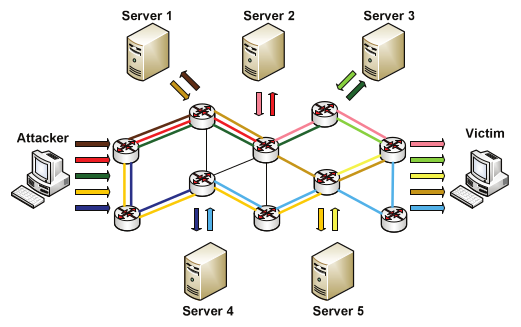
\includegraphics[width=0.7\textwidth]{Figures/rDoS}
\decoRule
\caption{Principe de dénie de service réflectif}
\label{fig:rDoS}
\end{figure} 

À ce niveau, on peut clairement voir que l'impact de ce type d'attaque est en double; en premier lieu, la consommation de la bande passante des liens réseau à cause du nombre excessif des messages requêtes et réponses échangés. En deuxième lieu, la surcharge des serveurs tiers avec des messages requêtes, qui vont les traiter évidemment, car pour eux ils paraissent des requêtes légitimes. 

\section{Motivation du travail}
Un article[\cite{24}] sur les travaux connexes a montré que la défense contre les attaques RDoS peut être divisée en 3 principales tâches : (1) surveillance (\textit{monitoring}) et la collecte de données du trafic réseau, (2) l’interprétation de ces données et la détection d’une attaque en cours, et (3) la mitigation de l’attaque. Selon leurs tâches principales, les solutions existantes varient considérablement dans leurs hypothèses et leurs exigences.\\
Dans la littérature on trouve que la surveillance du trafic, qui représente la première phase du processus de détection, se fait sur ces trois couches:\\
\begin{itemize}
\item[•] La couche réseau.
\item[•] La couche de transport.
\item[•] La couche d'application.\\
\end{itemize}
\newpage
Par exemple \textit{PacketScore}, par Kim et al [\cite{25}], utilise les statistiques de paquets collectés pour comparer chaque paquet reçu au trafic bénin et d’attaque pour ensuite lui attribuer une note. Les paquets qui sont similaires au trafic d’attaque sont éliminés. Cette approche nécessite une surveillance active de la couche réseau. Plusieurs autres travaux [\cite{26}, \cite{27}] s'intéressent à la couche de transport pour la détection des anomalies en analysant les paquets de transport, ICMP, TCP et UDP.\\

Pour cette fin, nous proposons une solution, basée sur une approche de clustering, pour la détection des ttaques Dos réflectives dans un réseau SDN. Cette solution prend en charge aussi les attaques DoS du type UDP-Flooding (voir section \ref{rdos}). La mitigation de l'attaque ne fait pas par partie de notre travail, on fera juste la détection. La première tâche, surveillance te collecte de données, va être lancée sur la couche de transport, où on surveillera spécialement le protocole de transport UDP, vu qu'il est le plus utilisé dans les attaques RDoS. Pour la deuxième phase, qui est la détection, on utilisera notre modèle d'apprentissage pour analyser les données collectées dans la phase précédente et décider si c'est une attaque ou non.

\section{Présentation de la Solution}
Les caractéristiques inhérentes des attaques de RDoS représentent un défi pour leur détection. Une surveillance et analyse continues du trafic réseau sont nécessaires pour la détection des flux malins. La solution qu'on propose, pour ce fait, est un système de détection, appelé \textbf{F-DoS}, qui sera déployée dans le réseau cible pour assurer la surveillance du trafic au but de détecter les attaques DoS (RDoS et UDP-Flooding).\\

Ces deux fonctions de surveillance et de détection sont assuré par deux modules intégrés dans notre système. Le premier est le module d'extraction d'informations, qu'on référencera par l'acronyme \textbf{MEI}. Une copie de chaque flux circulant dans le réseau est envoyée à ce module afin d'extraire ses caractéristiques. Les caractéristiques extraites sont ensuite envoyées au deuxième module de notre système, appelé \textbf{F-Clustering}, qui est un modèle intelligent, sa fonction est de grouper les flux en clusters, cluster des flux normaux et cluster des flux malins.\\

L'architecture et le principe de fonctionnement de notre système sont illustrés dans la figure suivante: \\

\begin{figure}[h]
\centering
\begin{minipage}[b]{.5\textwidth}
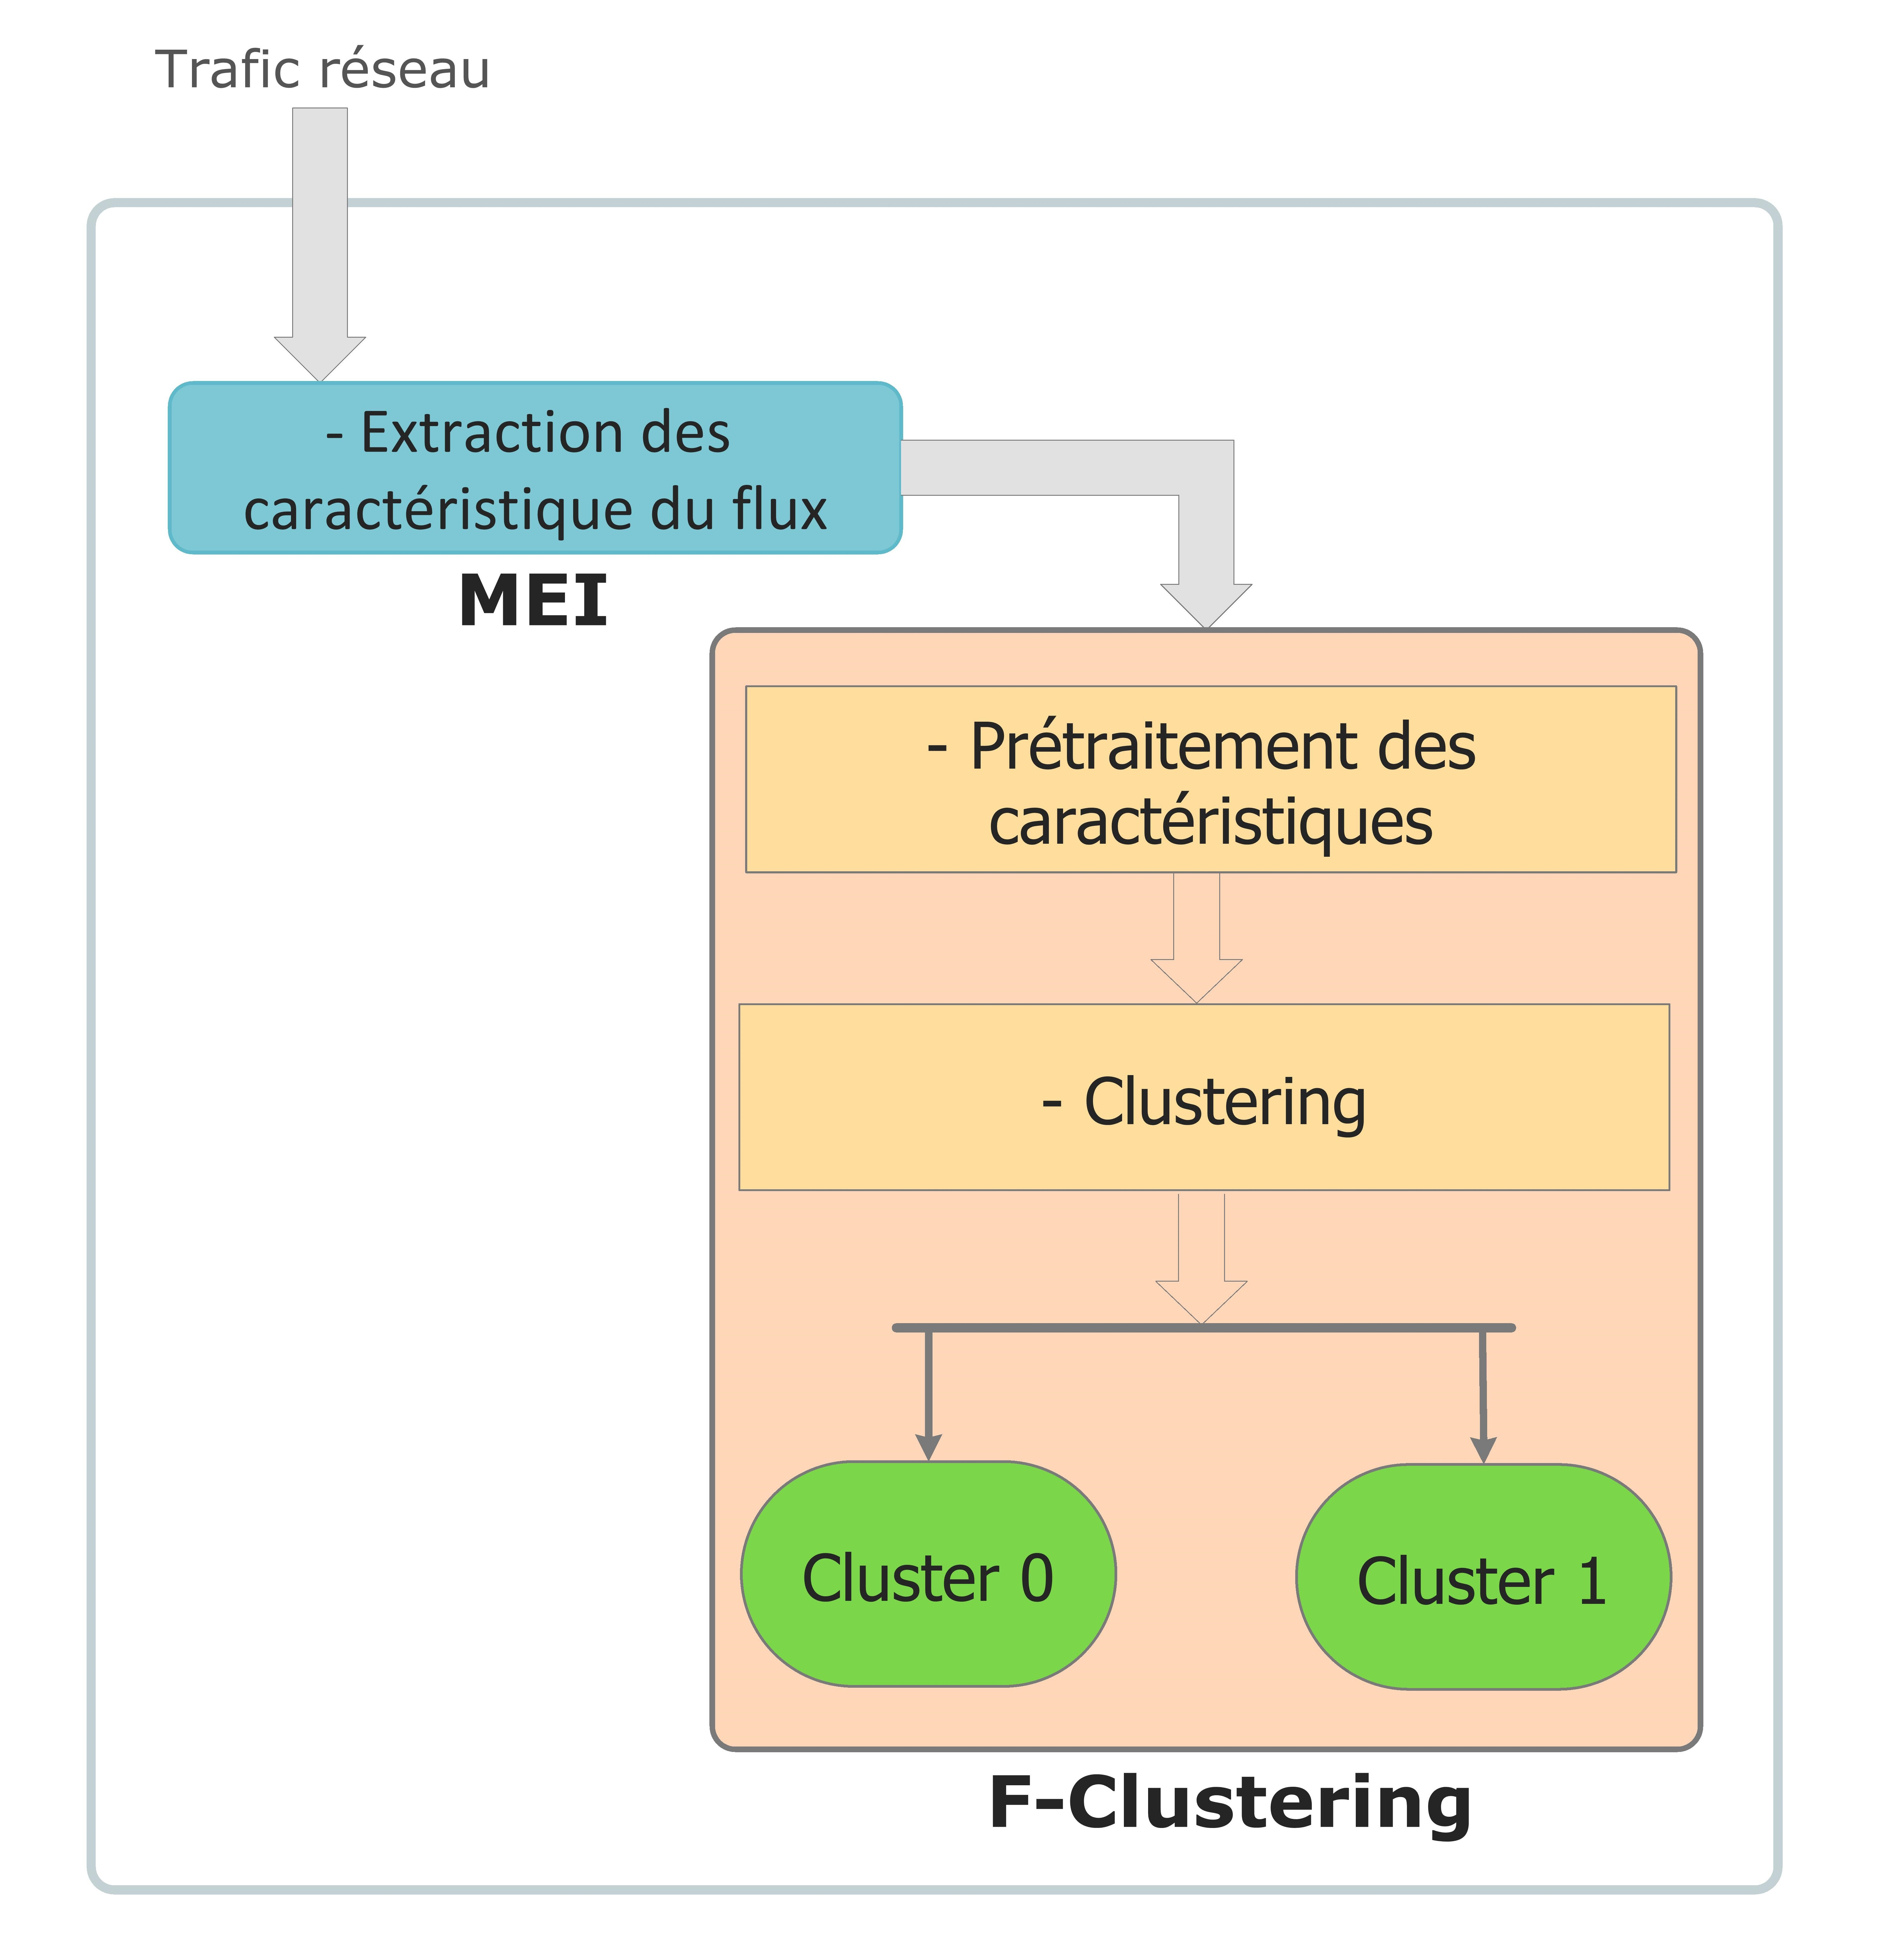
\includegraphics[width=\textwidth]{Figures/F-DoS}
\label{fig:rDoS}
\end{minipage}
\begin{minipage}[b]{.45\textwidth}
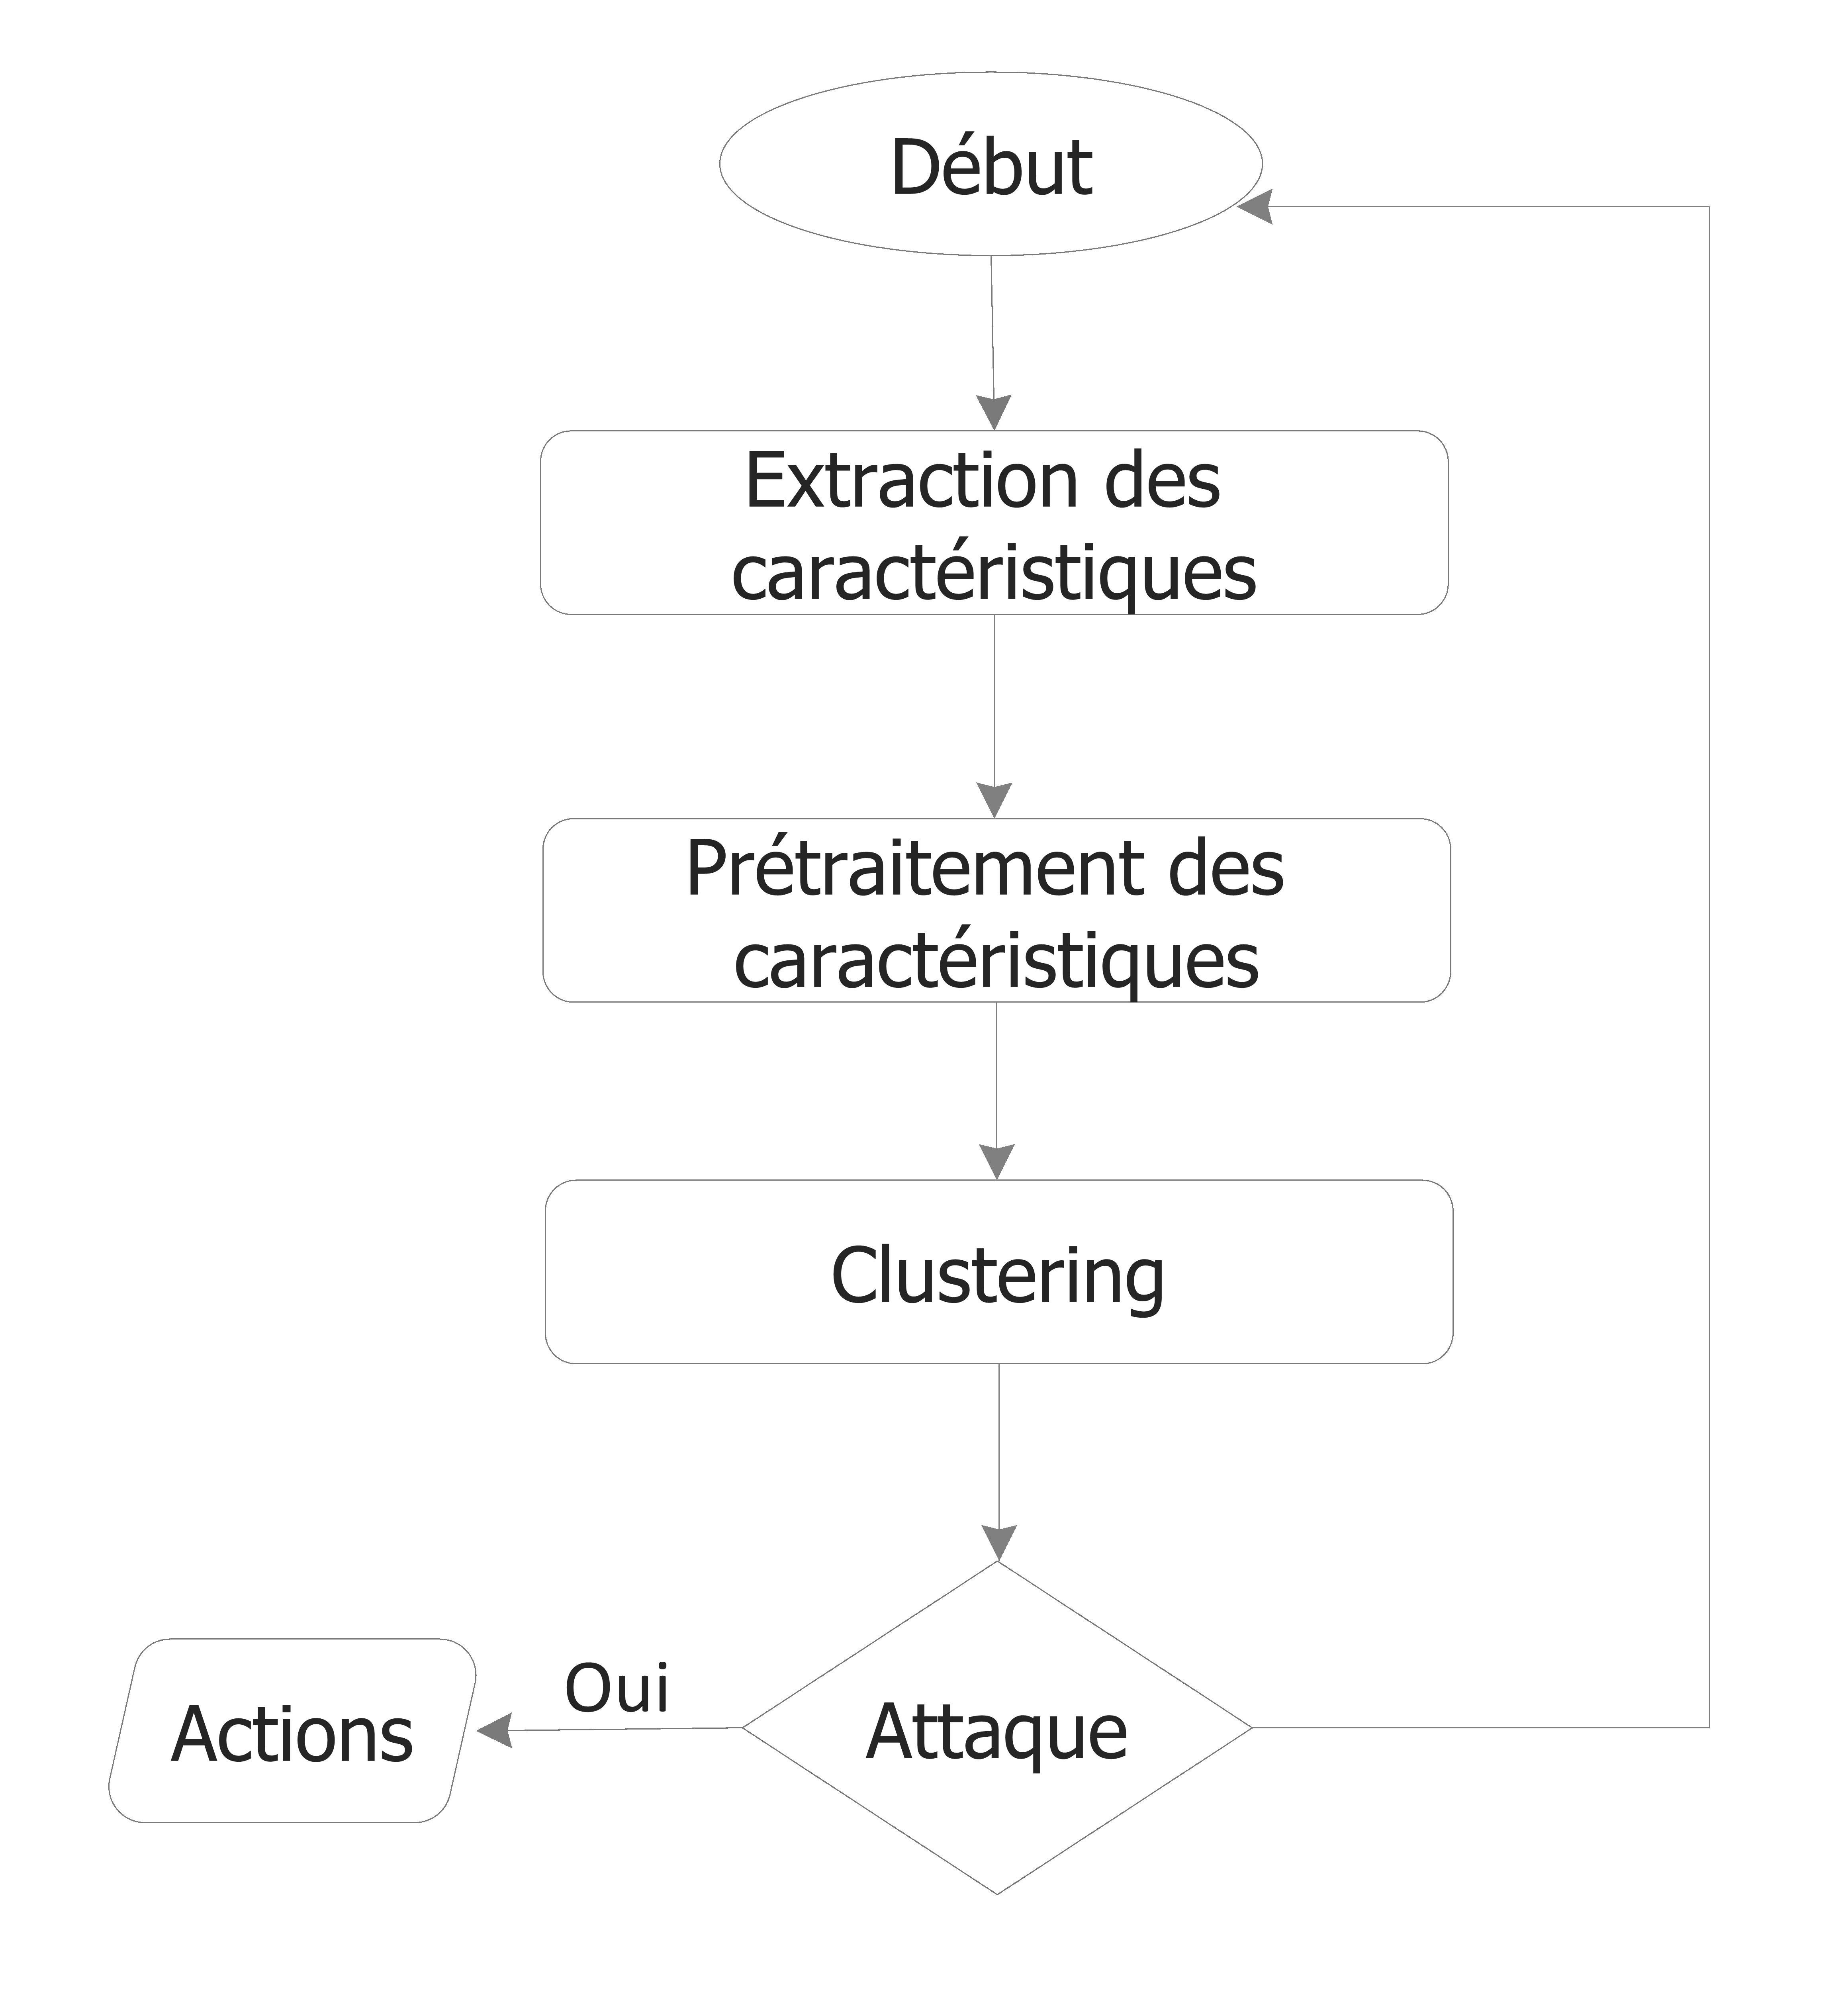
\includegraphics[width=\textwidth]{Figures/Diagramme}
\label{fig:rDoS}
\end{minipage}
\decoRule
\caption{Architecture et fonctionnemnt de F-DoS}
\end{figure}

\newpage
\subsection{Module MEI}
Le rôle principal de ce module est l'extraction des informations des flux de données. Mais pour ce faire, ce module doit assurer trois fonctions: l'écoute passive, l'analyse et l'extraction. Ce module à un port dédié à l'écoute, qui est toujours active pour recevoir une copie de chaque paquet à l'aide de la technique de mise en miroir \textit{Port Miroring}. L'ensemble des paquets capturés est envoyé par la suite à l'analyseur. L'analyse des paquets n'est pas une fonction simple, elle doit être effectuée soigneusement, si on analyse mal les paquets on risque de fausser le résultat de détection. Cette fonction est compliquée a raison que, l'analyseur reçoit tous les paquets qui circulent dans le réseau, et on a dit précédemant qu'on s'intéresse aux informations des flux de données, un flux est un ensemble de paquets qui partage le même \textit{Paquet Header}(c-a-d même adresse source, adresse destination, port, ... etc). Donc l'analyseur doit calculer les flux en regroupant les paquets communs, identifier les flux de données susceptibles et éliminer tout autre flux no intéressant, comme le flux des messages de contrôle, le flux des messages de sollicitation,...etc. Les flux de données formés vont ainsi être passés à la dernière fonction de ce module pour extraction de caractéristiques de chaque flux.

\newpage
\subsection{Module F-Clustering}
L'objet de notre travail est de proposer une approche de Clustering pour la détection des attaques Dos. On s'est penché vers le K-Means, nous l'avons amélioré et adapté à notre utilisation pour construire notre modèle intelligent qui est le coeur de ce module. Ce module prend en entrée le vecteur de caractéristiques construit par le module MEI, et d'après ses préconnaissances, et attribue le flux reçu a un des clusters préexistants. Si le flux est groupé dans le cluster des flux malin on dit qu'une attaque DoS (RDoS ou UDP-Flooding), on peut ainsi lancer une alerte et c'est à l'administrateur réseau de prendre action.

\section{Conception du module MEI}
Pour concevoir ce module, nous étions dans l’obligation de choisir un outil d’analyse et de calcul des caractéristiques des flux. Parmi les différents analyseurs existants, nous avons choisi ARGUS[\cite{31}] pour plusieurs raisons:\\
\begin{itemize}
\item[-] Son architecture client/serveur, est simple et personnalisable.
\item[-] Assure les trois fonctions de notre module MEI.
\item[-] Fonctionne en temps réel ce qui permet, par la suite, une détection d'attaques en temps réel.\\
\end{itemize} 
Pour mettre en oeuvre le module MEI, nous avons procédé comme suit:\\
\begin{itemize}
\item[1-] Premièrement, une copie du trafic réseau est redirigée vers ce module à l'aide du \textit{Port-Miroring} activé au niveau des \textit{switches}.\\
\item[2-] Un filtrage est appliqué pour supprimer tout paquet non intéressant pou ce travail.\\
\item[3-] Nous avons lancé le serveur ARGUS pour capturer les flux.\\
\item[4-] Nous avons lancé l’outil ARGUS-client, qui nous permet de sélectionner les caractéristiques et les informations des flux à extraire.\\
\item[5-] Nous traitons par la suite les informations collectées et nous les envoyons au module \textbf{F-Clustering}.\\
\end{itemize}

L'architecture interne du module MEI est illustrée dans la figure \ref{fig:MEI}
\begin{figure}[h]
\centering
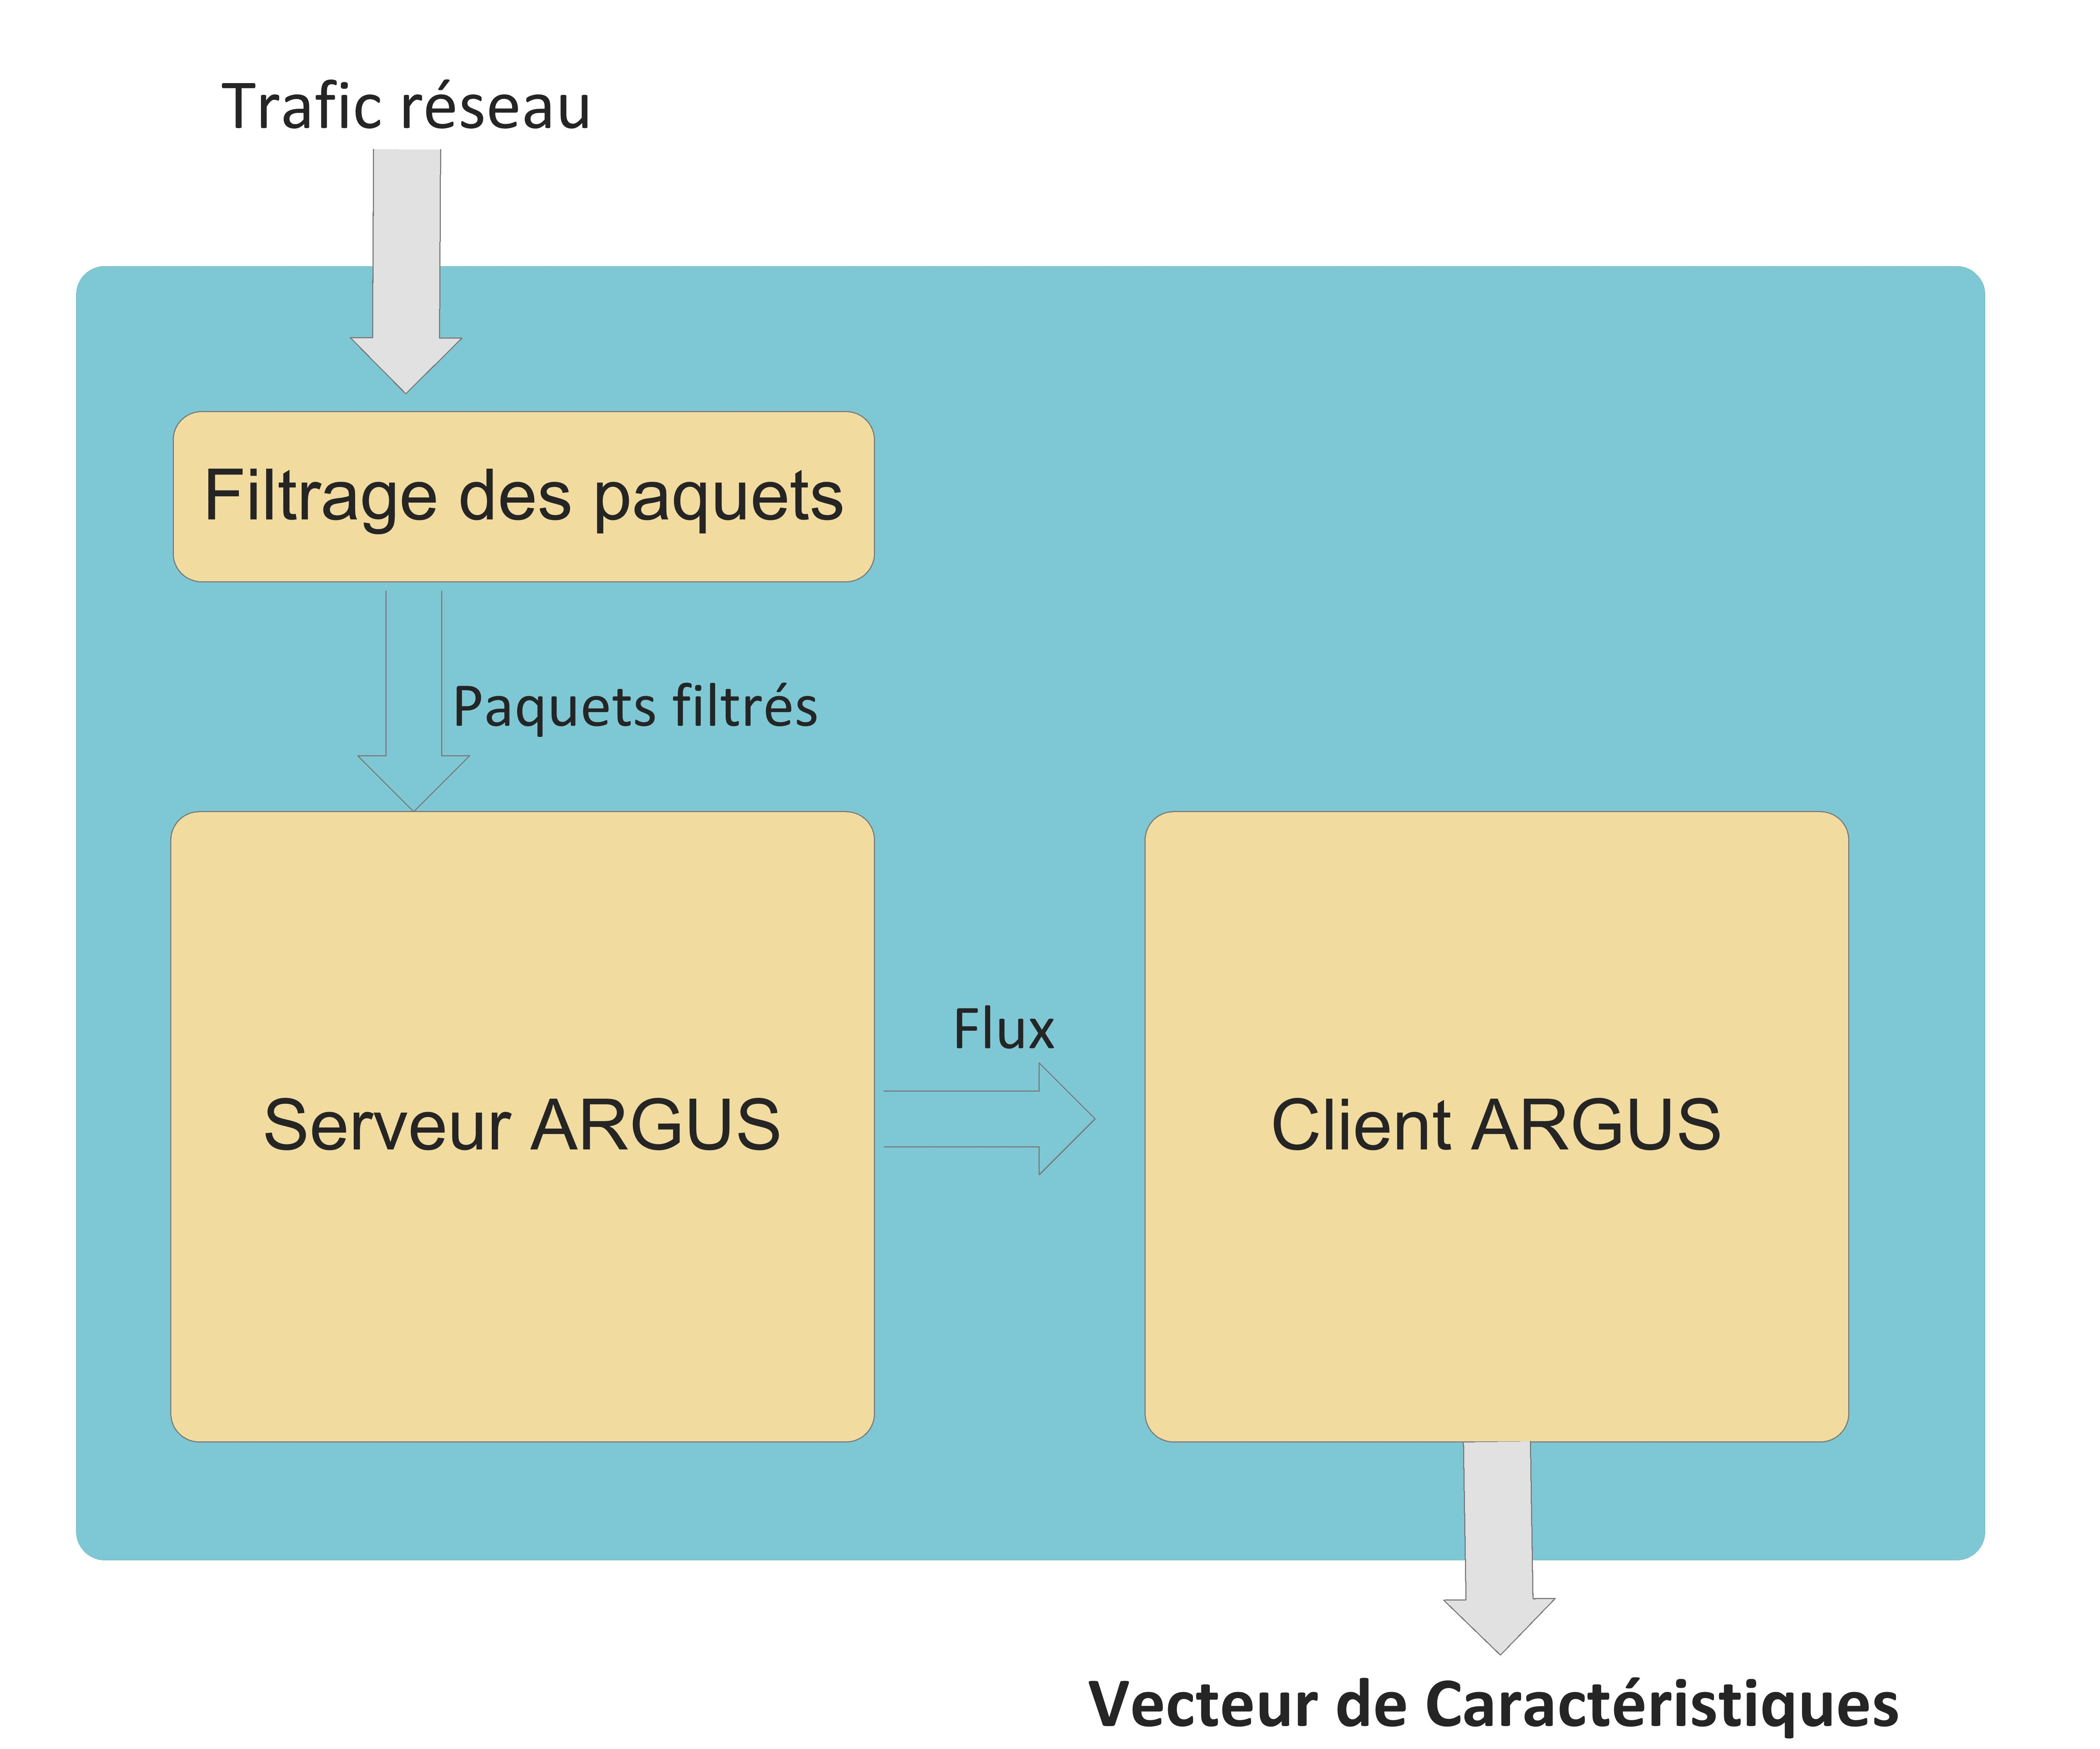
\includegraphics[width=0.6\textwidth]{Figures/MEI}
\decoRule
\caption{Architecture du module MEI}
\label{fig:MEI}
\end{figure} 

\newpage
\section{Conception du module F-Clustering}
\label{F-Clustering}
Pour concevoir ce module nous avons suivi les étapes du processus KDD décrites dans la section \ref{KDD}:\\
\begin{itemize}
\item[-] Préparation des données: premières étapes du processus, où on parlera de notre source donnée et les différentes opérations effectuées sur ces données pour les préparer à la deuxième phase du processus. \\
\item[-] Recherche du modèle: le modèle adopté est un modèle d'apprentissage non supervisé, utilisant une approche de Clustering, qui va être trainé sur les données collectées dans la phase précédente.\\
\item[-] Évaluation du modèle: on fera l'évaluation du modèle dans le chapitre \ref{Chapter5}.
\end{itemize}

\subsection{Préparation des données}
\subsubsection{A) Choix du dataset }
Comme source de données, nous avons exploité le dataset \textbf{ CICDDoS 2019}[\cite{21}]. CICDDoS2019 contient des flux bénins et des attaques Ddos les plus courantes, qui ressemblent aux vraies données du monde réel. Ce dataset contient différentes attaques DoS modernes réflectives telles que Portmap, Netbios, LDAP, UDP, TFTP, NTP. La période de capture a commencé le 12 janvier à 10 h 30 et s’est terminée à 17 h 15. Des attaques ont par la suite été exécutées au cours de cette période. \\

CICDDoS2019 est formé de plusieurs fichiers, chacun propre à une attaque. Vu la taille énorme de ces fichiers, et pour raison de simplifier le travail et pouvoir simuler l'architecture générale de notre réseau, on s'est mis d'accord sur le choix d'un seul fichier qu'on travaillera sur. Le fichier qu'on a choisi est propre à l'attaque TFTP, qui est lui-même un dataset contenant *** lignes et 87 colonnes (attributs).

\subsubsection{B) Prétraitement des données }
Le dataset TFTP n'est pas propre, il contient des données avec des ordres de grandeur différents, des valeurs erronées, des duplicats, il n'est pas balancé et contient des attributs qu'on n'a pas besoin dans notre travail. Un prétraitement est nécessaire pour préparer le dataset en vue de l'utiliser dans l'étape de création du modèle d'apprentissage. Ce processus de prétraitement est sur trois étapes; la première est le nettoyage du dataset, connue dans la littérature sous le nom de \textbf{Data Laundry}. Deuxième étape, sélection des attributs. Troisième étape, mise à l'échelle et balancement du dataset.

\subsubsection{B-1) Data Laundry}
Cette étape consiste à nettoyer le dataset:\\
\begin{itemize}
\item[-] Les lignes contenants des valeurs \textit{"Infinit"} ou \textit{"NaN"} seront supprimées.
\item[-] Suppression des duplicates.
\item[-] Les données vont être formatées en un \textit{datatype} standard.
\end{itemize}

\subsubsection{B-2) Sélection des attributs}
\label{attributs}
Dans notre travail, nous n'avons sélectionné que 10 attributs du dataset TFTP, que nous avons trouvé suffisant pour notre modèle d'apprentissage. Chaque attribut correspond à une caractéristique calculée par le module MEI, d'où le vecteur de caractéristiques généré par le module MEI est de taille 10 égale au nombre d'attributs sélectionnés. Le tableau suivant décrit chacun de ces attributs.\\

\begin{table}[h]
\begin{center}
\begin{tabular}{ | m{4cm} | m{10cm} | }
\hline
\rowcolor[rgb]{0.85,0.85,0.85}
\textbf{Attribut} & \textbf{Déscription}\\
\hline
Protocol & Protocol de transport\\
\hline
Flow Duration & Durée du flux\\
\hline
Total Fwd Packets & Nombre de paquets envoyées \\
\hline
Total Backward Packets &  Nombre de paquets reçus \\
\hline
Total Length of Fwd Packets & Taille totale des paquets envoyées \\
\hline
Total Length of Bwd Packets & Taille totale des paquets reçus \\
\hline
Flow Bytes/s &  Nombre de Byte par seconde\\ 
\hline
Flow Packets/s &  Nombre de paquets par seconde\\
\hline
Fwd Packets/s & Nombre de paquets envoyées par seconde \\
\hline
Bwd Packets/s & Nombre de paquets reçus par seconde \\
\hline
\end{tabular}
\caption{Déscription des attributs}
\label{table:attributs}
\end{center}
\end{table}

\newpage
\subsubsection{B-3) Mise à l'échelle et balancement}
La mise à l'échelle consiste à diminuer la grande différence entre les valeurs d'une même caractéristique C. Nous avons utilisé la technique Min-Max Scaler sur ce dataset, qui pour chaque valeur X applique l'opération suivante:
\begin{center}
{\large $ X_{scaled} = \frac{X - X_{min}}{X_{max} - X_{min}} $}
\end{center}
Où :\\
\indent X : valeur à mettre à l'échelle de la caractéristique C.\\
\indent $X_{min}$ : plus petite valeur observée de la caractéristique C. \\
\indent $X_{max}$ : plus grande valeur observée de la caractéristique C.\\

Le dataset TFTP n'est pas balancé, il contient beaucoup plus de flux attaqué que de flux bénin. Si on l'utilise sans le balancer, notre modèle va toujours pencher vers le cluster des attaques. L'idée du balancement est de générer de nouveaux échantillons de la classe minoritaire à l'aide de fonctions mathématiques existantes. On parlera sur la bibliothèque python utilisée pour le balancement du dataset dans le chapitre \ref{Chapitre5}.

\subsection{Recherche du modèle}
Deuxième étape du processus KDD. On a opté pour un modèle de Clustering, où a fait l'implémentation de l'algorithme K-Means avec des modifications pour l'adapter à notre utilisation. Le modèle prend en entrée le dataset construit dans l'étape de prétraitement, applique l'algorithme de clustering pour construire les deux clusters, attaque et bénin. En sortie, on aura un objet, qui groupe un flux donné dans un des clusters existants. Cet objet n'est rien d'autre que le module \textbf{F-Clustering} de notre système.
\begin{figure}[h]
\centering
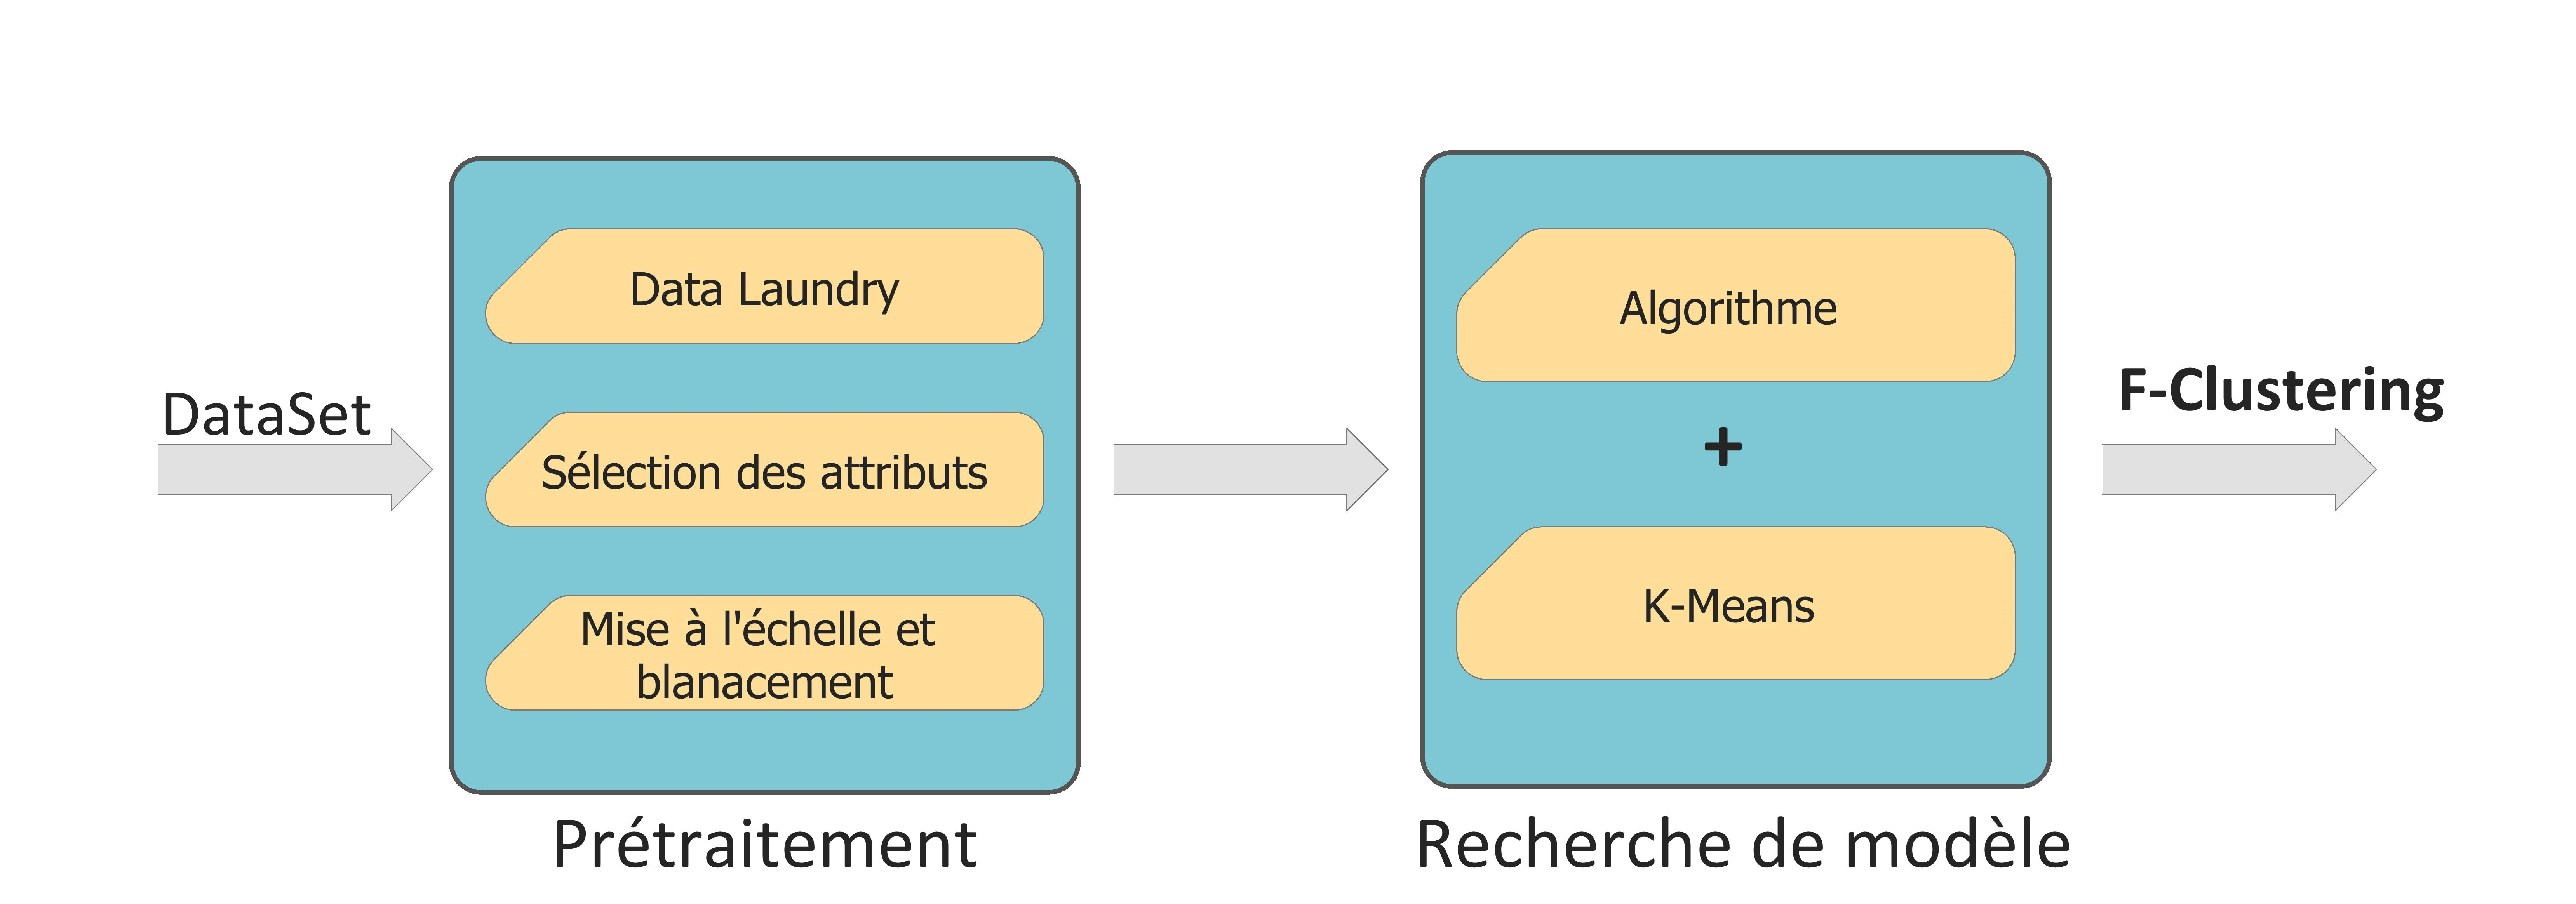
\includegraphics[width=\textwidth]{Figures/Diagramme2}
\decoRule
\caption{Étapes de conception de F-Clustering}
\label{fig:F-Clustering_Diagramme}
\end{figure} 

\section{Conclusion}
